\documentclass[11pt,reqno]{amsart}

\usepackage[utf8]{inputenc}
\usepackage[T1]{fontenc}
\usepackage{amsmath,amssymb,amsthm,mathtools}
\usepackage{geometry}
\geometry{a4paper, margin=1in}
\usepackage{hyperref}
\hypersetup{
    colorlinks=true,
    linkcolor=blue,
    citecolor=red,
    urlcolor=teal
}
\usepackage{tikz}
\usetikzlibrary{arrows.meta, calc}
\usepackage{microtype}
\usepackage{booktabs}
\usepackage{array}
\usepackage{tabularx}

% --- Teoremas e Estruturas ---
\newtheorem{theorem}{Theorem}[section]
\newtheorem{lemma}[theorem]{Lemma}
\newtheorem{proposition}[theorem]{Proposition}
\newtheorem{corollary}[theorem]{Corollary}
\newtheorem{conjecture}[theorem]{Conjecture}

\theoremstyle{definition}
\newtheorem{definition}[theorem]{Definition}
\newtheorem{remark}[theorem]{Remark}
\newtheorem{example}[theorem]{Example}
\newtheorem{assumption}[theorem]{Assumption}
\newtheorem{algorithm}[theorem]{Algorithm}

% --- Atalhos e Operadores ---
\providecommand{\R}{\mathbb{R}}
\newcommand{\N}{\mathbb{N}}
\newcommand{\C}{\mathbb{C}}
\providecommand{\II}{\mathrm{I\!I}}
\newcommand{\op}{\mathrm{op}}
\newcommand{\dist}{\mathrm{dist}}
\newcommand{\reach}{\mathrm{reach}}
\newcommand{\medial}{\mathcal{M}}
\providecommand{\Hsn}{\mathcal{H}}
\newcommand{\OmegaBar}{\bar{\Omega}}

\numberwithin{equation}{section}


\DeclareMathOperator*{\argmin}{argmin}
\providecommand{\Hyp}{\mathbb{H}}
\providecommand{\Sph}{\mathbb{S}}
\providecommand{\II}{\mathrm{II}}
\providecommand{\R}{\mathbb{R}}
\providecommand{\Area}{\mathrm{Area}}
\providecommand{\Hsn}{\mathcal{H}}
\providecommand{\BV}{\mathrm{BV}}
\providecommand{\TV}{\mathrm{TV}}
\providecommand{\cutnorm}[1]{\|#1\|_{\square}}

\begin{document}

\title[Minimax-Flat \texorpdfstring{$k$}{k}-Submanifolds in Obstacle Environments]{Minimax-Flat \texorpdfstring{$k$}{k}-Submanifolds in Obstacle Environments: Variational Theory, Constructive Heuristics, and Explicit Candidates}

\author{Reinaldo Maia Silva-Filho}
\address{Programa de P\'os-Gradua\c{c}\~ao em Estat\'istica e Experimenta\c{c}\~ao Agropecu\'aria (PPGEE/DES), Universidade Federal de Lavras (UFLA)}
\email{reinaldo.filho1@estudante.ufla.br}

\date{\today}

\begin{abstract}
We study the $L^\infty$ minimax curvature problem: among $k$-dimensional submanifolds $M^k$ of an obstacle domain $\bar{\Omega} \subset \R^n$ spanning a prescribed boundary $\Sigma^{k-1}$, minimize the peak normal curvature $\|\II_M\|_{L^\infty}$. We separate what can be proved from what cannot.

Proved results: (i) existence of $C^{1,1}$ minimizers for curves ($k=1$) with fixed endpoints, optional end tangents, obstacles and a length bound, by an Arzel\`a--Ascoli argument; (ii) a contact principle, valid for $C^{1,1}$ submanifolds and hence for the minimizers of (i): at an interior contact point with a $C^2$ obstacle boundary, the essential supremum of $\|\II_M\|_{\op}$ near the contact point is bounded below by the $k$-th principal curvature of $\partial\Omega$ measured towards $\Omega$; in particular, obstacle boundaries curving away from the free region impose no curvature \emph{at the contact point} (a line may touch a convex obstacle without bending), although such obstacles can still raise $\kappa^*$ by blocking straight competitors; (iii) elementary lower bounds (turning angle, the planar U-turn bound $2/w$, a Gauss--Bonnet floor for closed surfaces in any codimension) and a curvature gap of at least $2\pi/L$ between knotted embedded curves and immersed curves, from the F\'ary--Milnor theorem; (iv) dimensional monotonicity, a conditional lower bound for curves in $\C^m$ whose projections to the complex coordinate planes are curved, attained by a planar circle, and exact curvatures of explicit candidates (helices, cylinders, product tori), which give upper bounds.

We also give counterexamples to several natural-looking statements: a boundary curvature floor, a sagitta bound, the optimality of the cylinder spanning two circles, and an isotropy property of calibrated submanifolds. Regularity invariance, positivity of the saturated set, discrete $\Gamma$-convergence and the constructive pipeline are conjectures or heuristics.
\end{abstract}

\maketitle

\tableofcontents
\newpage

\section{Introduction and Problem Formulation}

\subsection{The \texorpdfstring{$L^\infty$}{L\textasciicircum\textbackslash{}infty} Variational Problem}
The variational theory of submanifolds spanning prescribed boundaries has historically focused on integral functionals. In the classical Plateau problem \cite{douglas1931}, area minimization yields minimal submanifolds with vanishing mean curvature ($H = 0$). In the Willmore problem \cite{willmore1965, simon1993, riviere2008}, one minimizes bending energy $\mathcal{W}(M) = \int_M H^2 \, dA$, and in elastic rope/rod theory, the total squared curvature $\int |\II|^2 \, dA$ is minimized \cite{langer1984}.

While these $L^1$ and $L^2$ functionals penalize average bending, they do not prevent localized curvature spikes. In several applications (maximum stress in thin shells, and path planning for vehicles with a bounded turning radius \cite{dubins1957, sussmann1995, chitsaz2007}) the relevant quantity is the \textbf{worst-case local bending}.

This motivates the \textbf{$L^\infty$ minimax curvature problem}:
\begin{equation}
\label{eq:variational_problem}
\kappa^*_{n,k,r}(V) := \inf_{M \in \mathcal{A}_r(\Omega, \Sigma, V)} \left\| \II_M \right\|_{L^\infty(M)}
\end{equation}
where:
\begin{itemize}
    \item $\Omega \subset \R^n$ is a bounded domain (the complement of the obstacles) with Lipschitz boundary $\partial\Omega$;
    \item $\Sigma^{k-1} \subset \partial\Omega$ is a compact, oriented smooth submanifold of dimension $k-1$ ($1 \le k < n$);
    \item $\II_M$ is the second fundamental form of $M^k \subset \R^n$;
    \item $\mathcal{A}_r(\Omega, \Sigma, V)$ is the admissible class of $C^r$-submanifolds $M^k \subset \bar{\Omega}$ with boundary $\partial M = \Sigma$ and volume $\Hsn^k(M) \le V$. We write $\mathcal{A}_{1,1}$ for the class of $C^{1,1}$ submanifolds.
\end{itemize}

\begin{remark}[Role of the volume bound]
\label{rem:compactness_necessity}
In this chapter $\Omega$ is bounded and the admissible class carries the bound $\Hsn^k(M) \le V$. If both were dropped, the problem would degenerate: for two points $p, q$ with prescribed end tangents, curves with arbitrarily small curvature exist in $\R^n$ once they are allowed to be arbitrarily long. Either assumption alone prevents this for curves. With the length bound this is Proposition~\ref{thm:lower_bounds}(1); if $\Omega \subset B(0,R)$ and a unit-speed curve has $|\kappa| \le \kappa < 1/R$, then $f = |\gamma|^2$ satisfies $f'' = 2 + 2\langle\gamma,\ddot\gamma\rangle \ge 2(1 - R\kappa) > 0$ and $0 \le f \le R^2$, which bounds the length of the curve. Boundaries of fractal type, where normals are undefined, are outside the scope of this chapter.
\end{remark}

\subsection{Topological Admissibility}
\label{subsec:embeddings_vs_immersions}
We fix a diffeomorphism class $[M_0]$ and consider two natural classes:
\begin{enumerate}
    \item \textbf{Embedded submanifolds:}
    \begin{equation}
    \mathcal{A}_r^{\mathrm{Emb}}(\Omega, \Sigma, V, [M_0]) := \left\{ M \in \mathcal{A}_r : M \cong [M_0] \text{ is an injective embedding} \right\}
    \end{equation}
    \item \textbf{Immersed submanifolds:}
    \begin{equation}
    \mathcal{A}_r^{\mathrm{Imm}}(\Omega, \Sigma, V, [M_0]) := \left\{ \iota: M^k \looparrowright \bar{\Omega} : \iota(M) \cong [M_0], \, d\iota_p \text{ has rank } k \, \forall p \in M \right\}
    \end{equation}
\end{enumerate}
For closed immersed surfaces in $\R^3$ with bounded area and bounded $\|\II\|_{L^p}$, $p > 2$, Langer's compactness theorem \cite{langer1985} shows that only finitely many diffeomorphism types occur, and Breuning \cite{breuning2015} extends this to immersions of arbitrary dimension and codimension with $\|\II\|_{L^\infty}$ bounded. For \emph{closed} submanifolds under a volume bound, fixing $[M_0]$ is therefore a normalization rather than a device against topological degeneration. Both theorems concern closed immersions; for the problem with prescribed boundary $\Sigma$ the finiteness does not follow directly from them (Remark after Proposition~\ref{thm:existence}).

Since $\mathcal{A}_r^{\mathrm{Emb}} \subset \mathcal{A}_r^{\mathrm{Imm}}$, the infima satisfy
\begin{equation}
\label{eq:embedding_immersion_gap}
\kappa^{*,\mathrm{Imm}}_{n,k,r}(\Omega, \Sigma, V, [M_0]) \le \kappa^{*,\mathrm{Emb}}_{n,k,r}(\Omega, \Sigma, V, [M_0]).
\end{equation}
The difference can be strictly positive when the embedded class also fixes an isotopy type.

\begin{proposition}[Knotting forces a curvature gap]
\label{prop:knot_gap}
Let $K$ be a nontrivial knot type in $\R^3$ and $L > 0$. Let $\kappa^*_K(L)$ be the infimum of $\|\kappa\|_{L^\infty}$ over closed $C^{1,1}$ embedded curves of knot type $K$ and length at most $L$, and $\kappa^*_{\mathrm{Imm}}(L)$ the same infimum over all closed immersed curves of length at most $L$. Then
\begin{equation}
\kappa^*_K(L) \ge \frac{4\pi}{L} = \kappa^*_{\mathrm{Imm}}(L) + \frac{2\pi}{L}.
\end{equation}
\end{proposition}

\begin{proof}
By the F\'ary--Milnor theorem \cite{milnor1950}, the total curvature of a knotted closed curve exceeds $4\pi$, so $4\pi < \int_0^\ell |\kappa|\,ds \le \ell\,\|\kappa\|_{L^\infty} \le L\,\|\kappa\|_{L^\infty}$. For immersed curves, the total curvature of any closed curve is at least $2\pi$ (Fenchel's theorem \cite{fenchel1929}), which gives $\|\kappa\|_{L^\infty} \ge 2\pi/L$, and the round circle of length $L$ attains $2\pi/L$. All closed immersed curves in $\R^3$ are regularly homotopic, so imposing a regular homotopy class does not change this infimum.
\end{proof}

\begin{remark}[Tie-breaking]
The $L^\infty$ functional is not strictly convex, and minimizers are in general not unique: a minimizer can often be modified where $\|\II\| < \kappa^*$. A natural selection rule picks, among minimizers, one of least volume. Whether such a secondary minimizer exists and is unique is not established here. (The area functional is not convex on spaces of submanifolds, so convexity arguments do not apply.)
\end{remark}

\begin{remark}[Scope of the constructive part]
The pipeline of Section~\ref{sec:pipeline} produces admissible candidates, and hence upper bounds on $\kappa^*$. We do not claim that it computes $\kappa^*$ exactly in any dimension, and we make no complexity claims.
\end{remark}

\subsection{Outline}
Section~2 fixes notation and relates the problem for planar curves to Dubins' shortest-path problem. Section~3 describes the heuristic constructive pipeline. Section~4 contains the contact principle and the lower bounds. Section~5 treats existence for curves, regularity, dimensional monotonicity and a conditional bound for curves curved in several planes. Section~6 computes explicit candidates. Section~7 discusses calibrated geometry and topological floors, and Section~8 summarizes the status of each claim.

\section{Geometric Framework, Operators, and Invariants}

\subsection{Differential Geometry of \texorpdfstring{$k$}{k}-Submanifolds in \texorpdfstring{$\R^n$}{R\textasciicircum n}}
Let $M^k \subset \R^n$ be an immersed $C^r$-submanifold ($r \ge 2$) with boundary $\partial M = \Sigma$. The ambient Euclidean connection is denoted by $\bar{\nabla}$.

\begin{definition}[Second Fundamental Form and Shape Operator]
For vector fields $X, Y \in \Gamma(TM)$ and normal field $\nu \in \Gamma(NM)$, the Gauss-Weingarten formulas are:
\begin{align}
\bar{\nabla}_X Y &= \nabla_X Y + \II(X, Y) \\
\bar{\nabla}_X \nu &= -A_\nu(X) + \nabla^\perp_X \nu
\end{align}
where $\nabla$ is the induced Levi-Civita connection on $M$, $\nabla^\perp$ is the connection on the normal bundle $NM$, $\II: TM \times TM \to NM$ is the symmetric bilinear \emph{second fundamental form}, and $A_\nu: TM \to TM$ is the self-adjoint \emph{shape operator} satisfying:
\begin{equation}
\langle A_\nu(X), Y \rangle_{\R^n} = \langle \II(X, Y), \nu \rangle_{\R^n}
\end{equation}
The eigenvalues $\kappa_1^\nu(p), \dots, \kappa_k^\nu(p)$ of $A_\nu$ are the principal curvatures along the normal direction $\nu \in S(N_pM) := \{\nu \in N_pM : |\nu|_{\R^n} = 1\}$.

The \emph{operator norm} of $\II_p$ is defined as:
\begin{equation}
\|\II_p\|_{\op} := \sup_{\substack{v \in T_pM \\ |v|=1}} |\II_p(v,v)|_{\R^n} = \max_{\nu \in S(N_pM)} \max_{i=1,\dots,k} |\kappa_i^\nu(p)|
\end{equation}
The global $L^\infty$-curvature functional of $M$ is:
\begin{equation}
\|\II_M\|_{L^\infty(M)} := \operatorname{ess\,sup}_{p \in M} \|\II_p\|_{\op}
\end{equation}
\end{definition}

By polarization, $\II(X,Y) = \frac12\big(\II(u,u) - \II(w,w)\big)$ with $u, w = (X \pm Y)/\sqrt2$, so $|\II(X,Y)| \le \|\II\|_{\op}$ for orthonormal $X, Y$. We use this in Proposition~\ref{prop:gauss_bonnet_floor}.

\subsection{Reach and Domain Regularity}
Obstacle constraints are conveniently described with Federer's reach \cite{federer1959}.
\begin{definition}[Reach and Medial Axis]
For a closed set $A \subset \R^n$, the \emph{medial axis} $\medial(A)$ is the set of points with at least two distinct closest points in $A$. The \emph{reach} is:
\begin{equation}
\reach(A) := \sup \left\{ \delta > 0 : \forall x \in \R^n \text{ with } \dist(x, A) < \delta, \, \exists ! \, \pi_A(x) \in A \right\}
\end{equation}
\end{definition}
Positive reach of the obstacle set $\R^n \setminus \Omega$ is a one-sided condition: it gives an exterior ball of radius $\reach(\R^n\setminus\Omega)$ at each boundary point, touching from the side of $\Omega$, but it allows corners pointing into $\Omega$. A convex polyhedral obstacle has infinite reach. Two-sided control is needed for regularity: if both $\R^n\setminus\Omega$ and $\bar\Omega$ have reach at least $\tau_0 > 0$, then $\partial\Omega$ satisfies a two-sided ball condition of radius $\tau_0$, hence is of class $C^{1,1}$ with principal curvatures bounded by $1/\tau_0$ a.e.\ (see, e.g., \cite{lewicka2020}).

\subsection{Planar Curves and Dubins Paths}
For curves in the plane, the minimax problem is dual to Dubins' problem \cite{dubins1957}. Fix oriented endpoints $(p, T_p)$ and $(q, T_q)$ in $\R^2$ without obstacles. For $\kappa > 0$, let $d_\kappa$ be the minimal length of a $C^{1,1}$ curve joining them with $|\kappa(s)| \le \kappa$ a.e. Dubins proved that minimizers exist and are concatenations of at most three pieces, each a circular arc of radius $1/\kappa$ or a segment, of type CSC or CCC. The function $\kappa \mapsto d_\kappa$ is nonincreasing, because the constraint becomes weaker as $\kappa$ grows.

\begin{proposition}[Dubins duality]
\label{prop:dubins_duality}
With this notation, the minimax curvature for curves of length at most $L$ joining the oriented endpoints is $\kappa^*(L) = \inf\{\kappa > 0 : d_\kappa \le L\}$. For $\kappa > \kappa^*(L)$, a Dubins path of curvature bound $\kappa$ is admissible and has curvature taking only the values $0$ and $\pm\kappa$.
\end{proposition}

\begin{proof}
If a curve of length at most $L$ has $\|\kappa\|_{L^\infty} \le \kappa$, then $d_\kappa \le L$. Hence $\kappa^*(L) \ge \inf\{\kappa : d_\kappa \le L\}$. Conversely, if $d_\kappa \le L$, the Dubins path for the bound $\kappa$ is admissible with peak curvature at most $\kappa$.
\end{proof}

In $\R^3$, Sussmann \cite{sussmann1995} derived necessary conditions for shortest paths with bounded curvature: they are of type CSC or CCC, or they contain helicoidal arcs. This is a structure result, not a complete classification. In $\R^n$ with $n \ge 3$, the curvature is a vector in the normal space rather than a scalar control, and the planar bang-bang structure does not transfer directly. For $k \ge 2$ we know of no analogue.

\section{A Heuristic Constructive Pipeline}
\label{sec:pipeline}

The following procedure produces admissible candidates, and hence upper bounds for $\kappa^*$. It is a design heuristic. We do not claim that it is optimal.

\begin{algorithm}[The $\mathcal{M}$-Minimax Constructive Pipeline]
\label{alg:constructive}
Given $\Omega \subset \R^n$, boundary $\Sigma^{k-1} \subset \partial\Omega$, and regularity $C^r$, a candidate $M$ is built in five steps.

\begin{enumerate}
    \item \textbf{Routing.}
    Compute the part $\medial(\R^n\setminus\Omega) \cap \Omega$ of the medial axis of the obstacle set that lies in the free region, and choose a homotopy class of $k$-dimensional subcomplexes of it, joined to $\Sigma^{k-1}$. Record the narrowest clearance
    \begin{equation*}
    w_{\min} = \inf_{x \in \text{path}} \dist(x, \partial\Omega).
    \end{equation*} For planar curves that must reverse direction inside a strip of width $w$, Proposition~\ref{thm:lower_bounds}(3) gives $\kappa^* \ge 2/w$. In higher dimensions no such bound follows from the clearance alone (Remark~\ref{rem:slab}).

    \item \textbf{Boundary relaxation (optional).}
    Suppose that, besides $\partial M = \Sigma$, a unit conormal field $\eta_0$ along $\Sigma$ is prescribed (the analogue of the end tangents of curves), i.e.\ the inward unit conormal $\eta_M$ of $M$ along $\Sigma$ must equal $\eta_0$. With noisy data, replace this exact condition by the penalty
    \begin{equation}
    \min_{M} \left\{ \|\II_M\|_{L^\infty} + \beta \int_\Sigma |\eta_M - \eta_0|^2 \, d\Hsn^{k-1} \right\},
    \end{equation}
    where $\beta$ has units of $L^{-k}$ so that both terms scale as inverse lengths.

    \item \textbf{Saturated pieces.}
    \begin{itemize}
        \item Curves ($k=1$): arcs of constant curvature (circles, helices) and segments, as in Proposition~\ref{prop:dubins_duality}.
        \item Hypersurfaces ($k=n-1$): pieces of hypercylinders $S^j(1/\kappa) \times \R^{n-1-j}$ and spheres $S^{n-1}(1/\kappa)$.
        \item Higher codimension: product tori and other submanifolds whose curvature is spread over several normal directions (Section~\ref{sec:examples}).
    \end{itemize}

    \item \textbf{Transitions.}
    Join pieces with transition layers. Clothoids $\kappa(s) = \kappa\,(s-s_0)/\Delta s$ give $C^2$ curves. A $C^r$ curve ($r \ge 3$) needs a curvature of class $C^{r-2}$, so a polynomial ramp from $0$ to $\kappa$ must have all derivatives of orders $1, \dots, r-2$ vanishing at both ends; together with the two end values these are $2(r-1)$ conditions, so the ramp has degree at least $2r-3$ (for $r = 3$, $\kappa(\tau) = \kappa\,(3\tau^2 - 2\tau^3)$, $\tau \in [0,1]$). The curvature of the transitions must stay below the target value.

    \item \textbf{Obstacle check.}
    Verify $M \subset \bar\Omega$. Contact is only possible at boundary points satisfying the necessary condition of Proposition~\ref{thm:obstacle_exclusion}, which applies to $C^{1,1}$ candidates by its item~(4).
\end{enumerate}
\end{algorithm}

\section{Contact Principle and Lower Bounds}

\begin{definition}[Curvature loci]
\label{def:loci}
For $M \in \mathcal{A}_{1,1}$ with $\|\II_M\|_{L^\infty} = \kappa^* > 0$, let $\|\II_p\|^*_{\op}$ be the precise representative of $p \mapsto \|\II_p\|_{\op}$, defined $\Hsn^k$-a.e. by Lebesgue averages. We call $\mathcal{F} = \{\|\II_p\|^*_{\op} = 0\}$ the \emph{flat locus}, $\mathcal{S} = \{\|\II_p\|^*_{\op} = \kappa^*\}$ the \emph{saturated locus}, $\mathcal{T} = \{0 < \|\II_p\|^*_{\op} < \kappa^*\}$ the \emph{transition locus}, and $\mathcal{B} = M \cap \partial\Omega$ the \emph{contact locus}.
\end{definition}

The sets $\mathcal{F}, \mathcal{S}, \mathcal{T}$ cover $M$ up to a null set by definition, while $\mathcal{B}$ may meet all of them.

\begin{conjecture}[Positive saturated measure]
\label{conj:saturated}
Suppose the obstacle constraint is \emph{active}, in the sense that $\kappa^*$ is strictly larger than the value of the same problem (same $\Sigma$, same volume bound, same boundary data) with $\bar\Omega$ replaced by $\R^n$. If a minimizer exists, then some minimizer has $\Hsn^k(\mathcal{S}) > 0$.
\end{conjecture}

\begin{remark}
The hypothesis of the conjecture excludes the obstacle-free case, but the analogous statement holds there for planar curves with prescribed end tangents. Let $\kappa^* > 0$ be the obstacle-free value for length at most $L$. By Proposition~\ref{thm:existence} some curve of length at most $L$ has curvature at most $\kappa^*$ a.e., so $d_{\kappa^*} \le L$. The Dubins path for the bound $\kappa^*$ is then admissible, hence a minimizer, and its curvature takes only the values $0$ and $\pm\kappa^*$. It is not a segment, since $\kappa^* > 0$, so it contains an arc of positive length on which $|\kappa| = \kappa^*$.
\end{remark}

\begin{proposition}[Contact principle]
\label{thm:obstacle_exclusion}
Let $\partial\Omega$ be of class $C^2$ near $p_0 \in \partial\Omega$, let $\nu$ be the unit normal at $p_0$ pointing into $\Omega$, and let $h$ be the second fundamental form of $\partial\Omega$ at $p_0$ with respect to $\nu$, with the sign convention that $h > 0$ when $\Omega$ is locally convex (for $\Omega$ a ball of radius $\rho$, $h = 1/\rho$; for the exterior of a ball, $h = -1/\rho$). Let $\lambda_1 \le \dots \le \lambda_{n-1}$ be the eigenvalues of $h$. Let $M \subset \bar\Omega$ be a $C^2$ submanifold and $p_0 \in M \cap \partial\Omega$ an interior point of $M$. Then:
\begin{enumerate}
    \item $T_{p_0}M \subset T_{p_0}\partial\Omega$, and $\langle \nu, \II_M(v,v) \rangle \ge h(v,v)$ for every $v \in T_{p_0}M$;
    \item $\|\II_M(p_0)\|_{\op} \ge \max\big(0, \lambda_k\big)$;
    \item if $U \subset \partial\Omega$ is closed, $\partial\Omega$ is $C^2$ near $U$ and $\lambda_k > \kappa$ at every point of $U$, then no $C^2$ submanifold $M \subset \bar\Omega$ with $\|\II_M\|_{L^\infty} \le \kappa$ touches $U$ at an interior point of $M$. If moreover $M$ is compact and $\partial M \cap U = \emptyset$, then $\dist(M, U) > 0$;
    \item items (2) and (3) hold for $C^{1,1}$ submanifolds $M \subset \bar\Omega$, in the form
    \begin{equation}
    \label{eq:contact_c11}
    \lambda_k(p_0) \le \lim_{r \to 0}\ \operatorname*{ess\,sup}_{p \in M \cap B(p_0, r)} \|\II_p\|_{\op} \le \|\II_M\|_{L^\infty}.
    \end{equation}
    In particular they apply to the minimizers of Proposition~\ref{thm:existence}.
\end{enumerate}
In particular, obstacle boundaries that curve away from $\Omega$ ($h \le 0$, e.g.\ convex obstacles) impose no curvature \emph{at the contact point}. They can still raise $\kappa^*$ by making straight or weakly curved competitors inadmissible: for $p = (-1,0)$, $q = (1,0)$ with end tangents $(1,0)$, the segment gives $\kappa^* = 0$ without obstacles, while a disk obstacle of radius $1/2$ centred at the origin excludes it, and then $\kappa^* \ge 1/2$. Indeed, let $\gamma$ be an admissible curve with $|\kappa| \le 1/2$ a.e.\ and tangent angle $\varphi$, $\varphi(0) = 0$. As long as $\cos\varphi > 0$, $\gamma$ is a graph $y(x)$ with $|d(\sin\varphi)/dx| = |\kappa| \le 1/2$, so $|\sin\varphi| \le (x+1)/2 < 1$ for $x < 1$. Hence $\gamma$ is a graph over the whole interval $[-1,1]$, and integrating $|dy/dx| = |\tan\varphi| \le u/\sqrt{4-u^2}$, $u = x+1$, gives $|y| \le 2 - \sqrt{4 - (x+1)^2}$. At $x = -1/4$ this is $|y| \le 0.15$, while the disk contains every point $(-1/4, y)$ with $|y| < 0.43$. So no admissible curve has $\|\kappa\|_{L^\infty} \le 1/2$. This bound needs no length constraint.
\end{proposition}

\begin{proof}
Let $d$ be the signed distance to $\partial\Omega$, positive in $\Omega$. It is $C^2$ near $p_0$ \cite[Lemma~14.16]{gilbarg2001}, with $\nabla d(p_0) = \nu$ and $\nabla^2 d(p_0)(v,v) = -h(v,v)$ for $v \in T_{p_0}\partial\Omega$. For a unit $v \in T_{p_0}M$ let $\alpha(t) = p_0 + tv + u(tv)$, where $u$ is the local graph function of $M$ over $T_{p_0}M$ used in the proof of (4) below. Since $p_0$ is interior to $M$, $\alpha$ is defined on an open interval, $\alpha(0) = p_0$, $\dot\alpha(0) = v$, and, $M$ being $C^2$, $\ddot\alpha(0) = D^2u(0)(v,v) = \II_M(v,v)$. (We do not use geodesics of $M$, whose existence is not automatic when the induced metric is only $C^1$.) The function $f = d \circ \alpha$ satisfies $f \ge 0$ and $f(0) = 0$, so $f$ has a local minimum at $0$. Then $\dot f(0) = \langle \nu, v\rangle = 0$, which gives $T_{p_0}M \subset \nu^\perp = T_{p_0}\partial\Omega$, and
\begin{equation}
0 \le \ddot f(0) = \nabla^2 d(p_0)(v,v) + \langle \nu, \II_M(v,v)\rangle = -h(v,v) + \langle \nu, \II_M(v,v)\rangle,
\end{equation}
which is (1). For (2), $\|\II_M(p_0)\|_{\op} \ge \max_{v \in T_{p_0}M,\,|v|=1} h(v,v) \ge \lambda_k$ by the Courant--Fischer min-max principle, since $T_{p_0}M$ is a $k$-dimensional subspace of $T_{p_0}\partial\Omega$. Item (3) follows from (2). If $M$ is compact and disjoint from the closed set $U$, their distance is positive.

For (4), let $M$ be $C^{1,1}$. The first-order argument above uses only $C^1$, so $T_{p_0}M \subset T_{p_0}\partial\Omega$. Near $p_0$ write $M$ as a graph $p_0 + y + u(y)$ over $y \in T_{p_0}M$, with $u \colon T_{p_0}M \to N_{p_0}M$ of class $C^{1,1}$, $u(0) = 0$, $Du(0) = 0$, and let $\delta(r) = \sup_{|y| < r}|Du(y)|$, so $\delta(r) \to 0$. Let $K_r$ be the essential supremum of $\|\II\|_{\op}$ on the part of $M$ over $\{|y| < r\}$. At a point $y$ where $D^2u(y)$ exists, the curve $t \mapsto p_0 + (y + tw) + u(y + tw)$ has acceleration $D^2u(y)(w,w) \in N_{p_0}M$, whose normal component at that point is $\II(w + Du(y)w, w + Du(y)w)$. Since the normal space there differs from $N_{p_0}M$ by $O(\delta(r))$,
\begin{equation*}
|D^2u(y)(w,w)| \le C_r\,|w|^2, \qquad C_r := K_r\,\frac{(1+\delta(r))^2}{1 - c\,\delta(r)},
\end{equation*}
for a.e.\ $|y| < r$, with a dimensional constant $c$. Let $g = \langle u, \nu\rangle$. Then $\partial_w^2 g \le C_r|w|^2$ a.e., hence also for the mollifications $g_\varepsilon$ of $g$, so $t \mapsto g_\varepsilon(tv) - \tfrac12 C_r t^2$ is concave; letting $\varepsilon \to 0$, the same holds for $g$. With $g(0) = 0$ and $\nabla g(0) = 0$ this gives $g(tv) \le \tfrac12 C_r t^2$ for $|t| < r$ and unit $v \in T_{p_0}M$. On the other hand, near $p_0$ the domain $\Omega$ lies on the side $\langle x - p_0, \nu\rangle \ge \varphi(x')$ of the graph of a $C^2$ function $\varphi$ over $T_{p_0}\partial\Omega$ with $\varphi(x') = \tfrac12 h(x',x') + o(|x'|^2)$. Since $M \subset \bar\Omega$ and the tangential part of $u(tv)$ is $O(t^2)$, we get $g(tv) \ge \tfrac12 h(v,v)t^2 + o(t^2)$. Comparing the two bounds as $t \to 0$ gives $h(v,v) \le C_r$ for every unit $v \in T_{p_0}M$, hence $\lambda_k \le C_r$ by Courant--Fischer, and \eqref{eq:contact_c11} follows as $r \to 0$. The analogue of (3) follows as before.
\end{proof}

\begin{remark}[Convex obstacles]
Neither $\|\II_{\partial\Omega}|_{TM}\|_{\op} \le \kappa^*$ at contact points, nor the impossibility of touching obstacle regions where $\|\II_{\partial\Omega}\|_{\op} > \kappa^*$, holds for convex obstacles: a straight line tangent to a ball of radius $\rho$ touches it with zero curvature, however large $1/\rho$ is. The sign of $h$, not its absolute value, controls contact.
\end{remark}

\begin{proposition}[Elementary lower bounds]
\label{thm:lower_bounds}
\leavevmode
\begin{enumerate}
    \item \textbf{Turning angle.} A curve of length at most $L$ with total turning $\Theta = \int_0^L |\kappa(s)|\,ds$ satisfies $\|\kappa\|_{L^\infty} \ge \Theta/L$.
    \item \textbf{Knotting.} See Proposition~\ref{prop:knot_gap}.
    \item \textbf{Planar U-turn.} A planar curve contained in a strip $\R \times [0,w]$ whose unit tangent turns from $(1,0)$ to $(-1,0)$ satisfies $\|\kappa\|_{L^\infty} \ge 2/w$, with equality for a semicircle of diameter $w$.
\end{enumerate}
\end{proposition}

\begin{proof}
(1) $\Theta = \int_0^L |\kappa|\,ds \le L\,\|\kappa\|_{L^\infty}$.
(3) This is proved in Chapter~8. We recall the argument. Let $\theta$ be a continuous tangent angle with $\theta(0) = 0$ and $\theta(L) \in \pi + 2\pi\mathbb{Z}$, and let $\kappa = \|\kappa\|_{L^\infty}$. There is a subinterval $[a,b]$ on which $\theta$ runs from $0$ to $\pm\pi$ and stays strictly between them, so $\sin\theta$ has constant sign on $(a,b)$. Since $|\dot\theta| \le \kappa$,
\begin{equation}
w \ge |y(b) - y(a)| = \int_a^b |\sin\theta|\,ds \ge \frac{1}{\kappa}\int_a^b |\sin\theta|\,|\dot\theta|\,ds \ge \frac{1}{\kappa}\,|\cos\theta(a) - \cos\theta(b)| = \frac{2}{\kappa}.
\end{equation}
\end{proof}

\begin{remark}[Bounds that fail]
\label{rem:slab}
\leavevmode
\begin{enumerate}
    \item[(a)] There is no \emph{boundary curvature floor} $\kappa^* \ge \sup_\Sigma \|\II_\Sigma\|_{\op}$. For $X$ tangent to $\Sigma$ at a point of $\Sigma$, $\II_\Sigma(X,X) = \II_M(X,X) + \II_{\Sigma \subset M}(X,X)$, with orthogonal summands, so $|\II_M(X,X)| \le |\II_\Sigma(X,X)|$; this controls $\II_M$ only in directions tangent to $\Sigma$ and only at points of $\Sigma$. The flat disk spanning a circle of radius $r$ has $\II_M = 0$ while $\|\II_\Sigma\| = 1/r$. The reverse inequality $\kappa^* \le \sup_\Sigma \|\II_\Sigma\|_{\op}$ fails as well: for $k = 1$, $\Sigma = \{p, q\}$ carries no curvature, while the U-turn of Proposition~\ref{thm:lower_bounds}(3) has $\kappa^* = 2/w > 0$. So there is no inequality between the two quantities in either direction.
    \item[(b)] The \emph{sagitta bound} $\kappa^* \ge 8d_{\min}/L^2$ fails. The circular arc with chord $L$ and sagitta $d$ has curvature $8d/(L^2 + 4d^2) < 8d/L^2$; for the semicircle ($d = L/2$) this is $2/L$, against $8d/L^2 = 4/L$.
    \item[(c)] The U-turn bound (3) is planar. In a slab $\{0 \le x_2 \le w\} \subset \R^3$ a curve can reverse direction by turning in the $x_1x_3$-plane, with $x_2$ constant, so the slab width gives no lower bound.
\end{enumerate}
\end{remark}

\begin{remark}[Homotopy classes and equioscillation]
The global value is the infimum of the values over homotopy classes of paths in $\Omega$. This is a tautology. Three further statements are natural but unproved: (i) every local minimizer contains arcs of exactly constant curvature $\kappa^*$ (``Chebyshev equioscillation''); (ii) $\kappa^*_{C^2} > \kappa^*_{C^{1,1}}$ strictly; (iii) winding loops are strictly suboptimal in the presence of an open half-space. Item (i) is stronger than Conjecture~\ref{conj:saturated}: it concerns every local minimizer and asks for arcs of constant curvature, whereas the conjecture asks only for one minimizer whose saturated locus has positive measure. Item (ii) fails as a statement about infima whenever the $C^{1,1}$ minimizer can be approximated by admissible $C^2$ curves with peak curvature at most $\kappa^* + \epsilon$, which we expect for Dubins paths without obstacles. What one expects instead is that the infimum over $C^2$ curves is not attained. Item (iii) is open.
\end{remark}

\section{Existence, Regularity, and Dimensional Effects}

\subsection{Existence for Curves}

\begin{proposition}[Existence of minimax curves]
\label{thm:existence}
Let $\bar\Omega \subset \R^n$ be closed, $p \ne q \in \bar\Omega$, $L \ge |p-q|$, and optionally fix unit end tangents $T_p, T_q$. If some $C^{1,1}$ curve in $\bar\Omega$ from $p$ to $q$ of length at most $L$ (with the prescribed tangents) exists, then the infimum $\kappa^*$ of $\|\kappa\|_{L^\infty}$ over such curves is attained.
\end{proposition}

\begin{proof}
Let $\gamma_j$ be a minimizing sequence, parametrized on $[0,1]$ proportionally to arc length, with lengths $\ell_j \in [|p-q|, L]$ and curvature bounds $\kappa_j \to \kappa^*$. Then $|\gamma_j'| = \ell_j$ and $\gamma_j'$ is Lipschitz with constant $\ell_j^2 \kappa_j \le L^2 \sup_j \kappa_j$. By Arzel\`a--Ascoli, a subsequence converges in $C^1$ to a curve $\gamma$ with $\ell_j \to \ell \ge |p-q| > 0$, $|\gamma'| \equiv \ell$, and $\mathrm{Lip}(\gamma') \le \liminf_j \ell_j^2\kappa_j = \ell^2\kappa^*$. Hence the arc-length reparametrization of $\gamma$ has curvature at most $\kappa^*$ a.e. The endpoints, the end tangents, the length bound and the constraint $\gamma \subset \bar\Omega$ are all preserved under $C^1$ convergence.
\end{proof}

\begin{remark}[Embeddedness and higher dimensions]
The limit of embedded curves may fail to be embedded, since two strands can touch in the limit. For $k \ge 2$, Langer's theorem \cite{langer1985} (closed surfaces in $\R^3$) and Breuning's extension \cite{breuning2015} (closed immersions in any dimension and codimension) give $C^{1,\alpha}$ subconvergence of sequences with bounded volume and bounded $\|\II\|_{L^\infty}$ after reparametrization, and the same lower semicontinuity argument then yields $C^{1,1}$ minimizers for closed immersed submanifolds in $\bar\Omega$ (the case $\Sigma = \emptyset$, which lies outside the formulation of Section~1). With a prescribed boundary $\Sigma$, a boundary version of this compactness would be needed, and we do not supply it.
\end{remark}

\subsection{Regularity}

\begin{conjecture}[Regularity invariance]
\label{thm:regularity_invariance}
Let $\Omega \subset \R^n$ be a bounded domain with $C^{1,1}$ boundary and $\Sigma^{k-1} \subset \partial\Omega$ compact and $C^\infty$. Then $\inf_{\mathcal{A}_r} \|\II\|_{L^\infty} = \inf_{\mathcal{A}_{1,1}} \|\II\|_{L^\infty}$ for every $r \ge 2$.
\end{conjecture}

\begin{remark}[Status]
The inequality $\ge$ is immediate from $\mathcal{A}_r \subset \mathcal{A}_{1,1}$. For the reverse, one mollifies a near-minimizer written as a normal graph over a smooth reference submanifold. Mollification does not increase $\|D^2 u\|_{L^\infty}$ and moves $Du$ uniformly little, so the curvature bound worsens only by $o(1)$. Three constraints must then be restored without losing this: the boundary condition $\partial M = \Sigma$, the volume bound, and the obstacle constraint when the near-minimizer touches $\partial\Omega$. We cannot do this in general, so the statement is a conjecture. For planar curves without obstacles we expect a direct proof from Proposition~\ref{prop:dubins_duality}, by smoothing the jumps in the curvature of a Dubins path and correcting the end conditions, but we have not written it out.
\end{remark}

\begin{remark}[Optimal regularity]
In the planar case without obstacles, minimizers of Dubins type are $C^{1,1}$, and their curvature jumps between $0$ and $\pm\kappa^*$, so they are not $C^2$. We expect $C^{1,1}$ to be the natural regularity class in general, by analogy with obstacle problems \cite{caffarelli1998}, but we have no proof.
\end{remark}

\subsection{Discretization}
Discrete Exterior Calculus \cite{hirani2003, crane2013} and discrete curvature energies \cite{wardetzky2007} suggest defining a discrete functional $\mathcal{F}_h$ on triangulations $\mathcal{T}_h$.

\begin{conjecture}[Discrete $\Gamma$-convergence]
\label{thm:dec_gamma_convergence}
There is a choice of discrete second fundamental forms for which $\mathcal{F}_h$ $\Gamma$-converges, as $h \to 0$, to $\|\II\|_{L^\infty}$ in a topology in which discrete minimizers are compact. Discrete minimizers then converge to continuous minimizers.
\end{conjecture}

\begin{remark}
In practice, obstacles smaller than the mesh size can be missed by vertex-based constraints. Refining the mesh near obstacles, for example with local size proportional to $\dist(x, \partial\Omega)$, is a standard remedy. It is a heuristic, not a theorem.
\end{remark}

\subsection{Dimensional Monotonicity and Curves Curved in Several Planes}

\begin{theorem}[Dimensional Monotonicity]
\label{thm:monotonicity}
Let $\Omega \subset \R^n$, $\Sigma \subset \partial\Omega$, and consider the canonical isometric embedding $i: \R^n \hookrightarrow \R^{n+1}$ given by $i(x) = (x, 0)$. Let $\tilde{\Omega} = \Omega \times (-d, d) \subset \R^{n+1}$ and $\tilde{\Sigma} = i(\Sigma)$. Then:
\begin{equation}
\kappa^*_{n+1, k, r}(\tilde{\Omega}, \tilde{\Sigma}, V) \leq \kappa^*_{n, k, r}(\Omega, \Sigma, V)
\end{equation}
\end{theorem}

\begin{proof}
For any $M \in \mathcal{A}_r(\Omega, \Sigma, V)$, the image $\tilde{M} = i(M) \subset \R^{n+1}$ is a $k$-submanifold with $\partial\tilde{M} = \tilde{\Sigma}$ and $\Hsn^k(\tilde{M}) = \Hsn^k(M) \le V$. Since $i$ is an affine isometry, second derivatives are mapped isometrically and the normal space of $\tilde M$ contains $i_*(N_pM)$, so $\|\tilde{\II}_{\tilde{M}}\|_{L^\infty} = \|\II_M\|_{L^\infty}$. Thus $\tilde{M} \in \mathcal{A}_r(\tilde{\Omega}, \tilde{\Sigma}, V)$, proving the inequality upon taking infima.
\end{proof}

\begin{figure}[htbp]
\centering
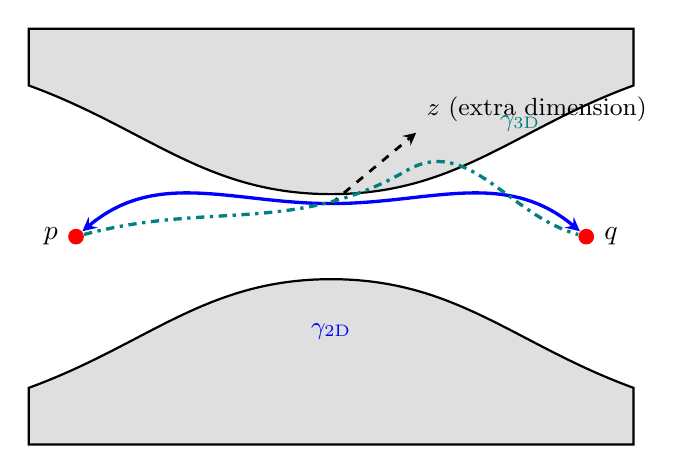
\begin{tikzpicture}[scale=1.2]
    \draw[fill=gray!25, draw=black, thick] (-3.2, 1.6) to[out=-20, in=180] (0, 0.45) to[out=0, in=200] (3.2, 1.6) -- (3.2, 2.2) -- (-3.2, 2.2) -- cycle;
    \draw[fill=gray!25, draw=black, thick] (-3.2, -1.6) to[out=20, in=180] (0, -0.45) to[out=0, in=-200] (3.2, -1.6) -- (3.2, -2.2) -- (-3.2, -2.2) -- cycle;
    \node[circle, fill=red, inner sep=2pt, label=left:{$p$}] (P) at (-2.7, 0) {};
    \node[circle, fill=red, inner sep=2pt, label=right:{$q$}] (Q) at (2.7, 0) {};
    \draw[very thick, blue, <->, >=stealth] (P) to[out=40, in=180] (0, 0.35) to[out=0, in=140] (Q);
    \node[blue, font=\small] at (0, -1.0) {$\gamma_{\text{2D}}$};
    \draw[dashed, ->, >=stealth, line width=1pt] (0, 0.35) -- (0.9, 1.1) node[above right, font=\small] {$z$ (extra dimension)};
    \draw[very thick, teal, dashdotted] (P) to[out=15, in=210] (0.8, 0.7) to[out=30, in=165] (Q);
    \node[teal, font=\small] at (2.0, 1.2) {$\gamma_{\text{3D}}$};
\end{tikzpicture}
\caption{Dimensional monotonicity: every admissible curve in $\R^n$ remains admissible in $\R^{n+1}$, so $\kappa^*$ cannot increase. Whether it strictly decreases depends on the configuration.}
\label{fig:monotonicity}
\end{figure}

\begin{proposition}[Curves curved in several planes; conditional]
\label{thm:scaling_law}
Write $\R^{2m} = \C^m$ with orthogonal projections $P_j$ onto the complex coordinate planes, and fix $R_0 > 0$.
\begin{enumerate}
    \item \textbf{Upper bound.} For any phases $\phi_j$, the curve $\gamma(s) = R_0 \sum_{j=1}^m \big( \cos(\omega s + \phi_j) \mathbf{e}_{2j-1} + \sin(\omega s + \phi_j) \mathbf{e}_{2j} \big)$ with $\omega = 1/(\sqrt m R_0)$ has unit speed and constant curvature $1/(\sqrt m R_0)$, and each projection $P_j\gamma$ is a circle of radius $R_0$. The curve itself is a planar circle of radius $\sqrt m R_0$.
    \item \textbf{Lower bound.} Let $\gamma \subset \C^m$ be a unit-speed $C^2$ curve such that, at each $s$ and for each $j$ with $v_j := P_j\dot\gamma(s) \ne 0$, the planar curve $P_j\gamma$ has curvature at least $1/R_0$. Then $|\ddot\gamma(s)| \ge 1/(\sqrt m R_0)$, with equality if and only if $|v_j|^2 = 1/m$ for all $j$ and each $P_j\ddot\gamma(s)$ is normal to $v_j$ with magnitude $|v_j|^2/R_0$.
\end{enumerate}
\end{proposition}

\begin{proof}
(1) In complex notation $\gamma(s) = R_0 e^{i\omega s} w$ with $w = \sum_j e^{i\phi_j}\mathbf{e}_j \in \C^m$, $|w|^2 = m$. As a real curve, $\gamma(s) = R_0(\cos(\omega s)\, w + \sin(\omega s)\, iw)$, and $w$, $iw$ are orthogonal real vectors of length $\sqrt m$, so $\gamma$ is a circle of radius $\sqrt m R_0$ in the real plane they span. Then $|\dot\gamma|^2 = m R_0^2\omega^2 = 1$ and $\ddot\gamma = -\omega^2\gamma$, so $|\ddot\gamma| = \omega^2 \sqrt m R_0 = 1/(\sqrt m R_0)$.
(2) The component of $P_j\ddot\gamma$ normal to $v_j$ has magnitude $\kappa_j |v_j|^2 \ge |v_j|^2/R_0$, where $\kappa_j$ is the curvature of $P_j\gamma$. Hence $|\ddot\gamma|^2 = \sum_j |P_j\ddot\gamma|^2 \ge R_0^{-2}\sum_j |v_j|^4 \ge R_0^{-2}\, m^{-1}\big(\sum_j |v_j|^2\big)^2 = (m R_0^2)^{-1}$ by Cauchy--Schwarz, since $\sum_j |v_j|^2 = 1$ for a curve in $\C^m$.
\end{proof}

\begin{remark}
The hypothesis in (2) is imposed and is not derived from an obstacle configuration. The extremal curve in (1) is a planar circle for every choice of phases; its curvature is spread over the $m$ complex coordinate planes only in the sense that each projection $P_j\gamma$ is curved. If $\gamma$ also moves in extra real directions ($n = 2m+1$), then $\sum_j |v_j|^2 \le 1$ and the bound weakens accordingly.
\end{remark}

% ==============================================================================
\section[Explicit Candidates in Low Dimensions]{Explicit Candidates in Low Dimensions \texorpdfstring{($n=2, 3, 4$)}{(n=2, 3, 4)}}
\label{sec:examples}
% ==============================================================================

The curvatures below are exact, and they give upper bounds for $\kappa^*$ in any configuration where the candidate is admissible. Optimality is proved only for the planar U-turn.

\subsection{Dimension \texorpdfstring{$n=2$}{n=2}: Planar Hairpin U-Turn \texorpdfstring{($k=1$)}{(k=1)}}
For a U-turn in the strip $\R \times [0,w]$, from tangent $(1,0)$ to tangent $(-1,0)$, the semicircle of radius $w/2$,
\begin{equation}
\gamma(s) = \left( \frac{w}{2} \sin\left(\frac{2s}{w}\right), \, \frac{w}{2}\Big(1 - \cos\left(\frac{2s}{w}\right)\Big) \right), \quad 0 \le s \le \frac{\pi w}{2}, \qquad \kappa = \frac{2}{w},
\end{equation}
is optimal by Proposition~\ref{thm:lower_bounds}(3). A $C^2$ transition from a segment is given by an Euler clothoid, with curvature $\kappa(s) = \kappa^* s/\Delta s$:
\begin{equation}
x(s) = \int_0^s \cos\left(\frac{\kappa^* t^2}{2 \Delta s}\right) dt, \quad y(s) = \int_0^s \sin\left(\frac{\kappa^* t^2}{2 \Delta s}\right) dt
\end{equation}

\subsection{Dimension \texorpdfstring{$n=3$}{n=3}: Helices and Cylinders \texorpdfstring{($k=1, 2$)}{(k=1, 2)}}
The circular helix
\begin{equation}
\gamma(s) = \left( a \cos\left(\frac{s}{c}\right), \, a \sin\left(\frac{s}{c}\right), \, \frac{b s}{c} \right), \quad c = \sqrt{a^2 + b^2},
\end{equation}
has curvature $\kappa = a/(a^2+b^2)$ and torsion $\tau = b/(a^2+b^2)$. With $a = R_0$ and $N$ turns over a height $H$ ($b = H/(2\pi N)$), this gives $\kappa = R_0/(R_0^2 + (H/2\pi N)^2) < 1/R_0$.

For $k=2$, the circular cylinder $X(u,\theta) = (R\cos\theta, R\sin\theta, u)$ spanning the circles $\{x^2+y^2 = R^2, z = 0\}$ and $\{x^2+y^2=R^2, z=H\}$ has shape operator $\operatorname{diag}(0, 1/R)$, so $\|\II\|_{\op} = 1/R$.

\begin{remark}[The cylinder is not optimal in general]
If the surface may bulge outwards, the cylinder can be beaten. The surface of revolution $r(z) = R + a\sin(\pi z/H)$ spans the same two circles. For $R = 1$, $H = 10$ its maximal principal curvature is $0.954$ for $a = 1$ and $0.728$ for $a = 3$, both below $1/R = 1$ (computed from the meridian curvature $|r''|/(1+r'^2)^{3/2}$ and the parallel curvature $1/(r\sqrt{1+r'^2})$; numerical check in the accompanying code repository). So $1/R$ is only an upper bound.
\end{remark}

\subsection{Dimension \texorpdfstring{$n=4$}{n=4}: Clifford Torus and Hypercylinders \texorpdfstring{($k=2, 3$)}{(k=2, 3)}}
For $k=2$, the flat Clifford torus $X(u, v) = \frac{R}{\sqrt{2}} (\cos u, \sin u, \cos v, \sin v)$ has metric $g = \frac{R^2}{2}(du^2 + dv^2)$. In the normal frame $\nu_1 = (\cos u, \sin u, 0, 0)$, $\nu_2 = (0,0,\cos v, \sin v)$, the shape operator along $\nu(\phi) = \cos\phi\, \nu_1 + \sin\phi\, \nu_2$ is
\begin{equation}
A_{\nu(\phi)} = -\frac{\sqrt{2}}{R} \begin{pmatrix} \cos\phi & 0 \\ 0 & \sin\phi \end{pmatrix}, \qquad \|\II\|_{\op} = \frac{\sqrt{2}}{R}
\end{equation}
(numerical check in the accompanying code repository). The torus is intrinsically flat. For $k=3$, the hypercylinder $S^2(R) \times \R$ has $A_\nu = \operatorname{diag}(1/R, 1/R, 0)$ and $\|\II\|_{\op} = 1/R$.

\section{Higher Dimensions, Calibrations, and Topological Floors}

\subsection{Families of Explicit Candidates}

\begin{table}[htbp]
\centering
\small
\renewcommand{\arraystretch}{1.15}
\begin{tabularx}{\textwidth}{@{}cc>{\raggedright\arraybackslash}p{3.1cm}>{\raggedright\arraybackslash}X>{\centering\arraybackslash}p{2.0cm}@{}}
\toprule
$n$ & $k$ & Candidate & Parametrization & $\|\II\|_{\op}$ \\
\midrule
$2$ & $1$ & Semicircle (U-turn, optimal) & radius $w/2$ & $\frac{2}{w}$ \\
$3$ & $1$ & Circular helix & $(a\cos\frac{s}{c}, a\sin\frac{s}{c}, \frac{bs}{c})$ & $\frac{a}{a^2+b^2}$ \\
$\ge 2m$ & $1$ & Diagonal circle (planar, radius $\sqrt m R_0$) & $R_0\sum_{j=1}^m e^{i(\omega s + \phi_j)}\mathbf{e}_j \in \C^m$ & $\frac{1}{\sqrt m R_0}$ \\
$\ge 2J\,(+1)$ & $1$ & General Frenet curve & $\sum_{j=1}^J r_j e^{i\omega_j s}\mathbf{e}_j$ (+ drift $\mathbf{d}\,s$ in an extra direction), $\sum_j r_j^2\omega_j^2 + |\mathbf{d}|^2 = 1$ & $\sqrt{\sum_j r_j^2\omega_j^4}$ \\
$n$ & $n-1$ & Hypercylinder & $S^{j}(R) \times \R^{n-1-j}$ & $\frac{1}{R}$ \\
$2m$ & $m$ & Product torus (Clifford for $m=2$, Lagrangian) & $\frac{R}{\sqrt m}(e^{iu_1}, \dots, e^{iu_m})$ & $\frac{\sqrt m}{R}$ \\
\bottomrule
\end{tabularx}
\caption{Explicit candidates and their exact peak curvatures. Except for the planar U-turn these are upper bounds in configurations where the candidate is admissible, not a classification of minimizers.}
\label{tab:universal_classification}
\end{table}

For the product torus with circles of radius $r = R/\sqrt m$, a unit tangent vector $v = \sum_j v_j \partial_{u_j}/r$ gives $|\II(v,v)|^2 = \sum_j v_j^4/r^2 \le 1/r^2$, with equality along a coordinate direction. Hence $\|\II\|_{\op} = \sqrt m/R$.

\begin{remark}[Two pitfalls]
First, the amplitude matters: the curve $\frac{R_0}{\sqrt m}\sum_j e^{i\omega s}\mathbf{e}_j$ has curvature $1/R_0$, not $1/(\sqrt m R_0)$: it is a circle of radius $R_0$. Second, the product $3$-torus in $\C^3$ is Lagrangian but not special Lagrangian: it is not minimal, and no compact minimal submanifold of $\R^n$ exists. We do not list candidates built from calibrated geometries, since we have no curvature values derived for them.
\end{remark}

\subsection{Calibrated Submanifolds}
Calibrated submanifolds in the sense of Harvey and Lawson \cite{harvey1982} are volume-minimizing in their homology class and in particular minimal ($H=0$). We know of no relation between calibration and the $L^\infty$ curvature problem.

\begin{remark}[Calibration does not force isotropy]
One might expect calibrated submanifolds to have ``vectorially isotropic'' second fundamental form, $\|\II\|_{\op} = \|\II\|_F/\sqrt{c}$ with $c = n-k$, and to minimize $\|\II\|_{\op}$ in their homology class. This fails already for complex curves in $\C^2$ ($k = c = 2$), which are calibrated by the K\"ahler form. There $\II(JX,Y) = J\,\II(X,Y)$ gives $\|\II\|_{\op} = \|\II\|_F/2$, not $\|\II\|_F/\sqrt2$. Indeed, in an orthonormal frame $(e_1, Je_1)$ one has $\II(e_1,e_1) = a$, $\II(e_1,Je_1) = Ja$ and $\II(Je_1,Je_1) = -a$, so $|\II(v,v)| = |a|$ for every unit $v$ while $\|\II\|_F = 2|a|$.
\end{remark}

\subsection{Topological Floors}

\begin{proposition}[Gauss--Bonnet floor for closed surfaces]
\label{prop:gauss_bonnet_floor}
Let $M^2 \subset \R^n$ be a closed $C^2$ surface of area $A$ and Euler characteristic $\chi$, with $\|\II_M\|_{L^\infty} \le \kappa$. Then
\begin{equation}
\kappa \ge \sqrt{\frac{2\pi\chi}{A}} \ \ \text{if } \chi > 0; \qquad \kappa \ge \sqrt{\frac{\pi|\chi|}{A}} \ \ \text{if } \chi < 0,
\end{equation}
and in codimension one ($n = 3$) the second bound improves to $\sqrt{2\pi|\chi|/A}$. The round sphere attains the first bound.
\end{proposition}

\begin{proof}
By the Gauss equation, $K = \langle \II(e_1,e_1), \II(e_2,e_2)\rangle - |\II(e_1,e_2)|^2$ in an orthonormal frame. Hence $K \le \kappa^2$, and, using $|\II(e_1,e_2)| \le \kappa$ (polarization), $K \ge -2\kappa^2$. In codimension one, $K = \kappa_1\kappa_2 \ge -\kappa^2$. The Gauss--Bonnet theorem $2\pi\chi = \int_M K\,dA$ then gives the bounds. For the sphere of radius $r$, $2\pi\cdot 2/(4\pi r^2) = 1/r^2$.
\end{proof}

\begin{remark}
In higher even dimension $2m$, the Gauss equation gives $|\mathrm{Rm}| \le C\kappa^2$, and the Gauss--Bonnet--Chern theorem yields $\kappa \ge c_m (|\chi|/\mathrm{Vol}(M))^{1/(2m)}$ for some constant $c_m > 0$. We do not know the optimal constant $c_m$.
\end{remark}

\section{Summary of Status}
\label{sec:status}
Proved here: Propositions~\ref{prop:knot_gap}, \ref{prop:dubins_duality}, \ref{thm:obstacle_exclusion}, \ref{thm:lower_bounds}, \ref{thm:existence}, \ref{thm:scaling_law}, \ref{prop:gauss_bonnet_floor} and Theorem~\ref{thm:monotonicity}, together with the exact curvatures of the candidates in Section~\ref{sec:examples} and Table~\ref{tab:universal_classification}. The contact principle holds for $C^{1,1}$ submanifolds (Proposition~\ref{thm:obstacle_exclusion}(4)), so it applies to the minimizers of Proposition~\ref{thm:existence}; it constrains the curvature only at contact points, and obstacles that curve away from $\Omega$ can still raise $\kappa^*$. Classical inputs: Dubins, F\'ary--Milnor, Fenchel, Langer--Breuning, Gauss--Bonnet. Open: Conjectures~\ref{conj:saturated}, \ref{thm:regularity_invariance} and \ref{thm:dec_gamma_convergence}, existence for $k \ge 2$ with prescribed boundary, optimality of every candidate except the planar U-turn, and any analogue of the Dubins structure for $k \ge 2$. The constructive pipeline (Algorithm~\ref{alg:constructive}) is a heuristic.

% Shared declarations block, \input by every chapter before its bibliography.
% Keep in sync with the "Declarations" section of master_book_unified_quantum_gravity.tex.
\section*{Declarations}

\noindent\textbf{Funding.} This research was financed in part by the Coordena\c{c}\~ao de Aperfei\c{c}oamento de Pessoal de N\'ivel Superior -- Brasil (CAPES) -- Finance Code 001.

\medskip\noindent\textbf{Competing interests.} The author declares no competing interests.

\medskip\noindent\textbf{Use of generative AI tools.} Large language model assistants (Anthropic Claude; Google Gemini, used through the Antigravity agent environment) were used extensively in preparing this work: drafting and editing text and \LaTeX{} source; proposing, expanding and revising derivations and proofs under the author's direction; writing the Python verification scripts and the \textsc{Lean 4} files; searching and checking the literature and references; and adversarial auditing of proofs, numerical claims and code. These audits found errors, some of them originally introduced with AI assistance. The errors and their corrections are recorded in the repository file \texttt{WORKPLAN.md}. AI tools are not authors. The author chose the research questions and the overall framework, reviewed the material, and is responsible for the content, including any remaining errors.

\medskip\noindent\textbf{Verification status.} Results labelled Theorem, Proposition or Lemma are proved in the text or cited as classical; statements labelled Conjecture are not proved. The numerical scripts compare formulas of the text with independent computations and are checks, not proofs. The \textsc{Lean 4} modules in \texttt{formal\_proofs\_book/Book} are a naming skeleton and do not verify the mathematics of this chapter.

\medskip\noindent\textbf{Code and data availability.} Sources, numerical scripts and the audit log are available at
\begin{center}\url{https://github.com/reinaldomsilvafilho-netizen/quantum-gravity-lean4}.\end{center}
The monograph is archived on Zenodo, \href{https://doi.org/10.5281/zenodo.22290043}{doi:10.5281/zenodo.22290043}, under the CC~BY~4.0 license.


\begin{thebibliography}{99}

\bibitem{douglas1931}
J.~Douglas,
\emph{Solution of the problem of Plateau},
Trans. Amer. Math. Soc. \textbf{33} (1931), no. 1, 263--321, \href{https://doi.org/10.1090/s0002-9947-1931-1501590-9}{doi:10.1090/s0002-9947-1931-1501590-9}.

\bibitem{willmore1965}
T.~J.~Willmore,
\emph{Note on embedded surfaces},
An. \c{S}tiin\c{t}. Univ. ``Al. I. Cuza'' Ia\c{s}i Sec\c{t}. I a Mat. \textbf{11} (1965), 493--496.

\bibitem{riviere2008}
T.~Rivi\`ere,
\emph{Analysis aspects of Willmore surfaces},
Invent. Math. \textbf{174} (2008), no. 1, 1--45, \href{https://doi.org/10.1007/s00222-008-0129-7}{doi:10.1007/s00222-008-0129-7}.

\bibitem{dubins1957}
L.~E.~Dubins,
\emph{On curves of minimal length with a constraint on average curvature, and with prescribed initial and terminal positions and tangents},
Amer. J. Math. \textbf{79} (1957), 497--516, \href{https://doi.org/10.2307/2372560}{doi:10.2307/2372560}.

\bibitem{sussmann1995}
H.~J.~Sussmann,
\emph{Shortest 3-dimensional paths with a prescribed curvature bound},
Proceedings of the 34th IEEE Conference on Decision and Control (1995), 3306--3311, \href{https://doi.org/10.1109/cdc.1995.478997}{doi:10.1109/cdc.1995.478997}.

\bibitem{chitsaz2007}
H.~Chitsaz and S.~M.~LaValle,
\emph{Time-optimal paths for a Dubins airplane},
Proceedings of the 46th IEEE Conference on Decision and Control (2007), 2379--2384, \href{https://doi.org/10.1109/cdc.2007.4434966}{doi:10.1109/cdc.2007.4434966}.

\bibitem{federer1959}
H.~Federer,
\emph{Curvature measures},
Trans. Amer. Math. Soc. \textbf{93} (1959), 418--491, \href{https://doi.org/10.1090/s0002-9947-1959-0110078-1}{doi:10.1090/s0002-9947-1959-0110078-1}.

\bibitem{langer1984}
J.~Langer and D.~A.~Singer,
\emph{The total squared curvature of closed curves},
J. Differential Geom. \textbf{20} (1984), no. 1, 1--22, \href{https://doi.org/10.4310/jdg/1214438990}{doi:10.4310/jdg/1214438990}.

\bibitem{langer1985}
J.~Langer,
\emph{A compactness theorem for surfaces with $L_p$-bounded second fundamental form},
Math. Ann. \textbf{270} (1985), no. 2, 223--234, \href{https://doi.org/10.1007/bf01456183}{doi:10.1007/bf01456183}.

\bibitem{breuning2015}
P.~Breuning,
\emph{Immersions with bounded second fundamental form},
J. Geom. Anal. \textbf{25} (2015), no. 2, 1344--1386, \href{https://doi.org/10.1007/s12220-014-9472-7}{doi:10.1007/s12220-014-9472-7}.

\bibitem{milnor1950}
J.~W.~Milnor,
\emph{On the total curvature of knots},
Ann. of Math. \textbf{52} (1950), no. 2, 248--257, \href{https://doi.org/10.2307/1969467}{doi:10.2307/1969467}.

\bibitem{gilbarg2001}
D.~Gilbarg and N.~S.~Trudinger,
\emph{Elliptic Partial Differential Equations of Second Order},
Classics in Mathematics, Springer, Berlin, 2001, \href{https://doi.org/10.1007/978-3-642-61798-0}{doi:10.1007/978-3-642-61798-0}.

\bibitem{fenchel1929}
W.~Fenchel,
\emph{\"Uber Kr\"ummung und Windung geschlossener Raumkurven},
Math. Ann. \textbf{101} (1929), 238--252, \href{https://doi.org/10.1007/BF01454836}{doi:10.1007/BF01454836}.

\bibitem{lewicka2020}
M.~Lewicka and Y.~Peres,
\emph{Which domains have two-sided supporting unit spheres at every boundary point?},
Expo. Math. \textbf{38} (2020), no. 4, 548--558, \href{https://doi.org/10.1016/j.exmath.2019.01.003}{doi:10.1016/j.exmath.2019.01.003}.

\bibitem{caffarelli1998}
L.~Caffarelli,
\emph{The obstacle problem revisited},
J. Fourier Anal. Appl. \textbf{4} (1998), no. 4-5, 383--402, \href{https://doi.org/10.1007/bf02498216}{doi:10.1007/bf02498216}.

\bibitem{simon1993}
L.~Simon,
\emph{Existence of surfaces minimizing the Willmore functional},
Comm. Anal. Geom. \textbf{1} (1993), no. 2, 281--326, \href{https://doi.org/10.4310/cag.1993.v1.n2.a4}{doi:10.4310/cag.1993.v1.n2.a4}.

\bibitem{harvey1982}
R.~Harvey and H.~B.~Lawson,
\emph{Calibrated geometries},
Acta Math. \textbf{148} (1982), 47--157, \href{https://doi.org/10.1007/bf02392726}{doi:10.1007/bf02392726}.

\bibitem{hirani2003}
A.~N.~Hirani,
\emph{Discrete Exterior Calculus},
Ph.D. thesis, California Institute of Technology, 2003, \href{https://doi.org/10.7907/ZHY8-V329}{doi:10.7907/ZHY8-V329}.

\bibitem{crane2013}
K.~Crane, F.~de Goes, M.~Desbrun, and P.~Schr{\"o}der,
\emph{Digital Geometry Processing with Discrete Exterior Calculus},
ACM SIGGRAPH 2013 courses, 1--126, \href{https://doi.org/10.1145/2504435.2504442}{doi:10.1145/2504435.2504442}.

\bibitem{wardetzky2007}
M.~Wardetzky, M.~Bergou, D.~Harmon, D.~Zorin, and E.~Grinspun,
\emph{Discrete quadratic curvature energies},
Computer Aided Geometric Design \textbf{24} (2007), no. 8--9, 499--518, \href{https://doi.org/10.1016/j.cagd.2007.07.006}{doi:10.1016/j.cagd.2007.07.006}.

\end{thebibliography}

\end{document}
